\documentclass[letterpaper,12pt]{article}
\usepackage[utf8]{inputenc}

\usepackage{rotating}
\usepackage[top=1in, bottom=1in, left=1in, right=1in]{geometry}
\usepackage{graphicx}
\usepackage[numbers,square,sort&compress]{natbib}
\usepackage{setspace}
\usepackage[cdot,mediumqspace,]{SIunits}
\usepackage{hyperref}
\usepackage{mathtools}
\usepackage{url}
\usepackage{authblk}
\usepackage{placeins}
\usepackage{float}

\onehalfspacing
\title{PHY254 Computational Assignment 2013}
\author{Anita Bahmanyar}
%\affil{\small {anita.bahmanyar@mail.utoronto.ca}}
%\affil{\small {anita.bahmanyar@mail.utoronto.ca}}
\date{November 30, 2013}

\usepackage{graphicx}

\renewcommand\thesubsection{\alph{subsection}}

\begin{document}

\maketitle

\section{The Rossler System}
\label{sec:therosslersystem}

%secion A
\subsection{}
The Rossler system is a set of coupled, first order, nonlinear ODEs that can exhibit chaos. It is defined by the equations of motion:
\begin{equation}
\frac{dx}{dt}=-y-z
\end{equation}

\begin{equation}
\frac{dy}{dt}=x+ay 
\end{equation}

\begin{equation}
\frac{dz}{dt}=b+ z(x-c)
\end{equation}

The initial values are to be set to:
a=0.1, b=0.1, c=2, x(0)=y(0)=z(0)=10.0 and time step is supposed to be 0.001.The following equations are the Rossler system equations using approximation:

\begin{equation}
x(t+\Delta t) = (-y-z)\Delta t +x(t)
\end{equation}

\begin{equation}
y(t+\Delta t) = (x+ay)\Delta t + y(t)
\end{equation}

\begin{equation}
z(t+\Delta t) = (b+z(x-c))\Delta t + z(t)
\end{equation}

In the code I wrote, instead of \begin{math} x(t+\Delta t) \end{math}, I used \begin{math} x_{i+1} \end{math} so that it iterates the i values each time using a while loop. Here is bait of my code:

\\*delta-t=0.001
\\*time-array= np.arange(0,100,delta-t)
\\*nt=len(time-array)
\\*x = np.zeros(nt)
\\*y =np.zeros(nt)
\\*z= np.zeros(nt)
\\*x[0]=10.0
\\*y[0]=10.0
\\*z[0]=10.0
\\*i=0
\\*while i < nt-1:
   \\* x[i+1]=((-y[i]-z[i])*delta-t)+x[i]
    \\*y[i+1]=((x[i]+(a*y[i]))*delta-t)+y[i]
    \\*z[i+1]=((b+(z[i]*(x[i]-c)))*delta-t)+z[i]
    \\*i+=1
\\*plt.plot(time-array,x)


\FloatBarrier
\begin{figure}[h!]
\centering
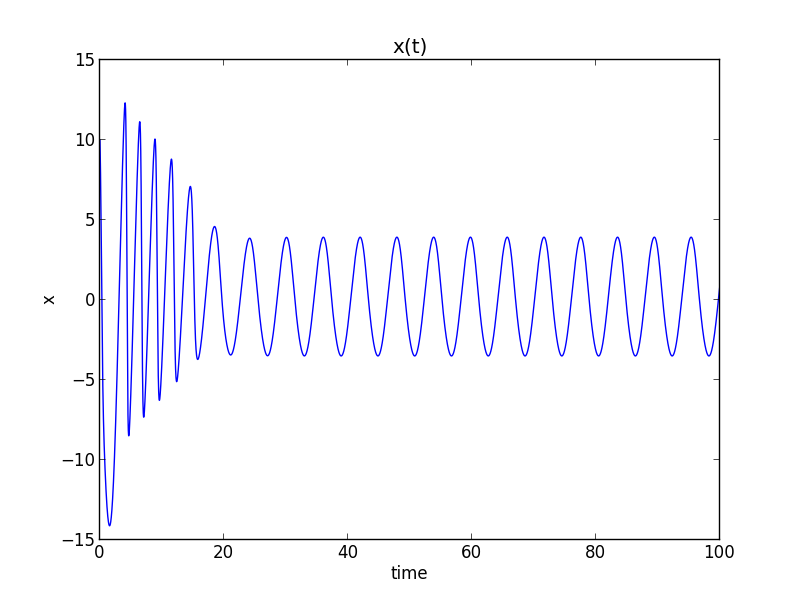
\includegraphics[scale=0.6]{1_a.png}
\caption{x(t) from Rossler System}
This figure shows x(t) from the Rossler system for the first 100 seconds of the system evolution. Here a=0.1, b=0.1, c=2, x(0)=y(0)=z(0)=10.0 with time step of 0.001
\end{figure}
\FloatBarrier

%section B
\subsection{}
Here, I used the same code as in part a and only changed the c value to be 4(other initial conditions have the same value as before).
We would say the that this system has approximately collapsed onto an attractor when the motion becomes periodic(not chaotic). When the motion of the system is chaotic, it does not follow any special path or pattern. For instance, here with these initial conditions, we say it has collapsed to attractor at about time t=23.
\FloatBarrier
\begin{figure}[h~]
\centering
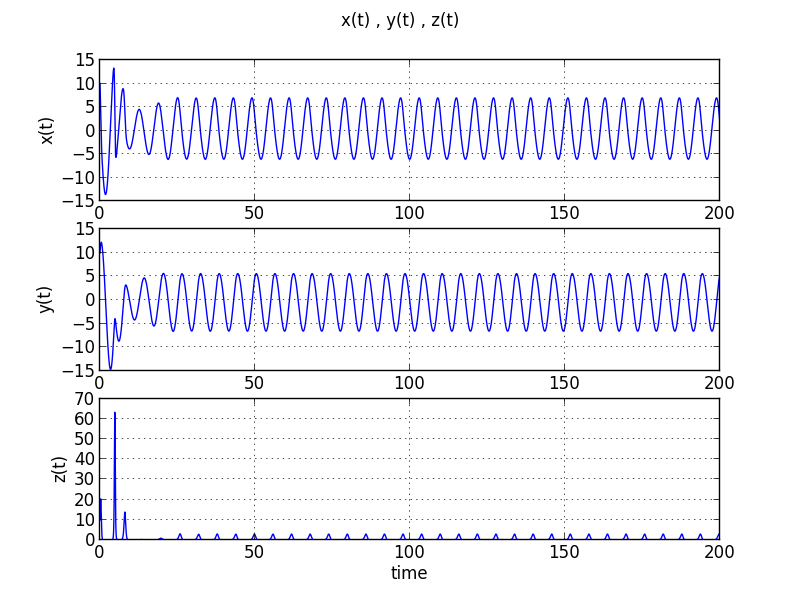
\includegraphics[scale=0.7]{1_b.png}
\caption{x(t) from Rossler System}
This figure shows x(t), y(t) and z(t) from the Rossler system for the first 200 seconds of the system evolution. Here a=0.1, b=0.1, c=4, x(0)=y(0)=z(0)=10.0 with time step of 0.001
\end{figure}
\FloatBarrier

%secion C
\subsection{}
As it is seen in the figures 3,4 and 5,  as the c value increases, the time it takes for the system to repeat also increases. This means that as c value increases, the system moves onto its attractor later, therefore the system spends more time being chaotic.
%c=4 image
\FloatBarrier
\begin{figure}[h!]
\centering
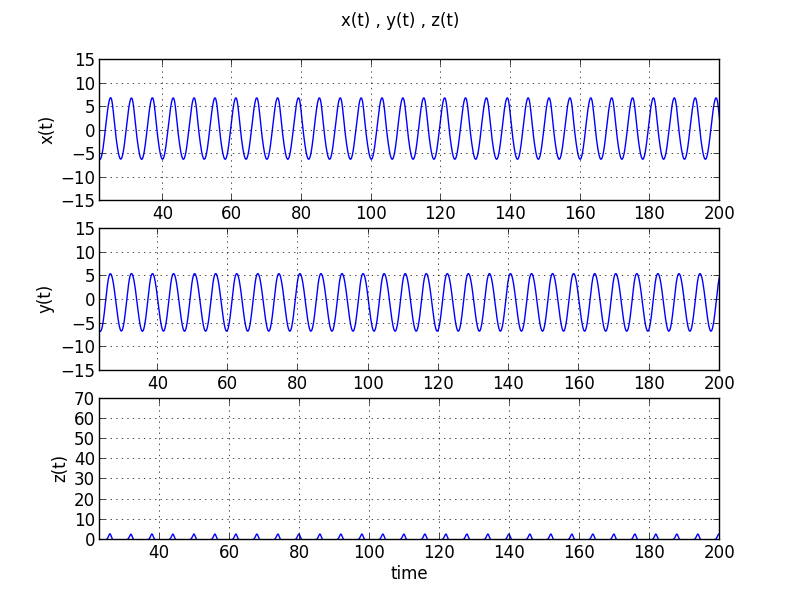
\includegraphics[scale=0.7]{1_c_4.png}
\caption{x(t) from Rossler System}
This figure shows x(t), y(t) and z(t) from the Rossler system for time after the system has evolved to attractor until 200 seconds. Here a=0.1, b=0.1, c=4, x(0)=y(0)=z(0)=10.0 with time step of 0.001
\end{figure}
\FloatBarrier

%c=6.5
\FloatBarrier
\begin{figure}[h!]
\centering
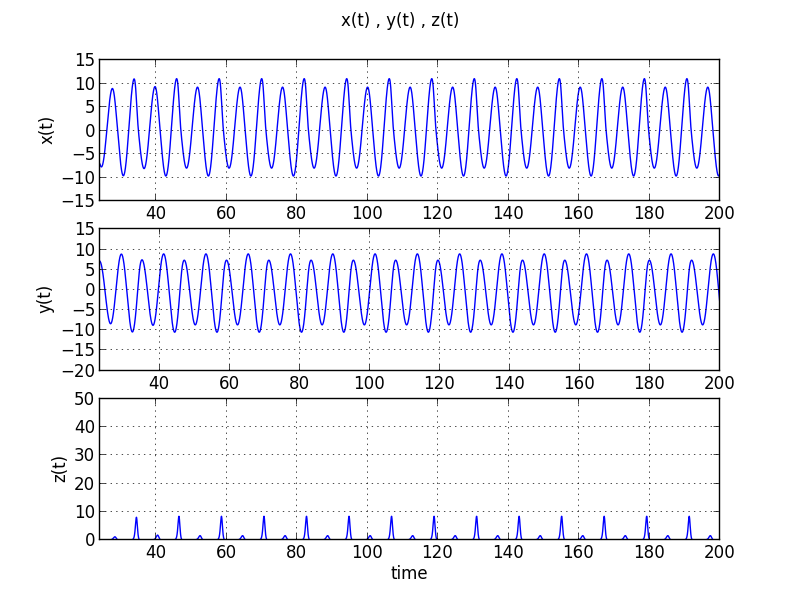
\includegraphics[scale=0.7]{1_c_6.png}
\caption{x(t) from Rossler System}
This figure shows x(t), y(t) and z(t) from the Rossler system for time after the system has evolved to attractor until 200 seconds. Here a=0.1, b=0.1, c=6.5, x(0)=y(0)=z(0)=10.0 with time step of 0.001

\end{figure}
\FloatBarrier

%c=8
\FloatBarrier
\begin{figure}[h!]
\centering
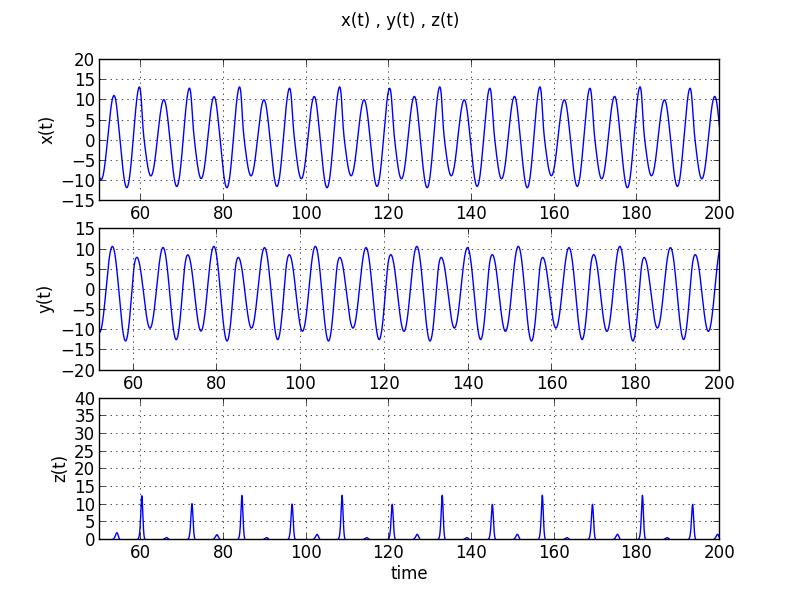
\includegraphics[scale=0.7]{1_c_8.png}
\caption{x(t) from Rossler System}
This figure shows x(t), y(t) and z(t) from the Rossler system for time after the system has evolved to attractor until 200 seconds. Here a=0.1, b=0.1, c=8, x(0)=y(0)=z(0)=10.0 with time step of 0.001
\end{figure}
\FloatBarrier


\subsection{}
Figure 6 shows the bifurcation diagram for about 120 values of c between 4 and 15 with the time step of 0.01 s. The first 250 seconds of the simulation is discarded in order to make sure that the solution is on the attractor. The very dense regions correspond to chaotic regions of parameter space. What bifurcation diagram does is that it adds another frequency to the system, so the system would be more chaotic. If there is infinite number of frequencies added to the system, the system would never repeat itself so it would be always chaotic. When another frequency is added to the system, the diagram splits in two at a certain point if is it doubling period as it is doing here.

\FloatBarrier
\begin{figure}[h!]
\centering
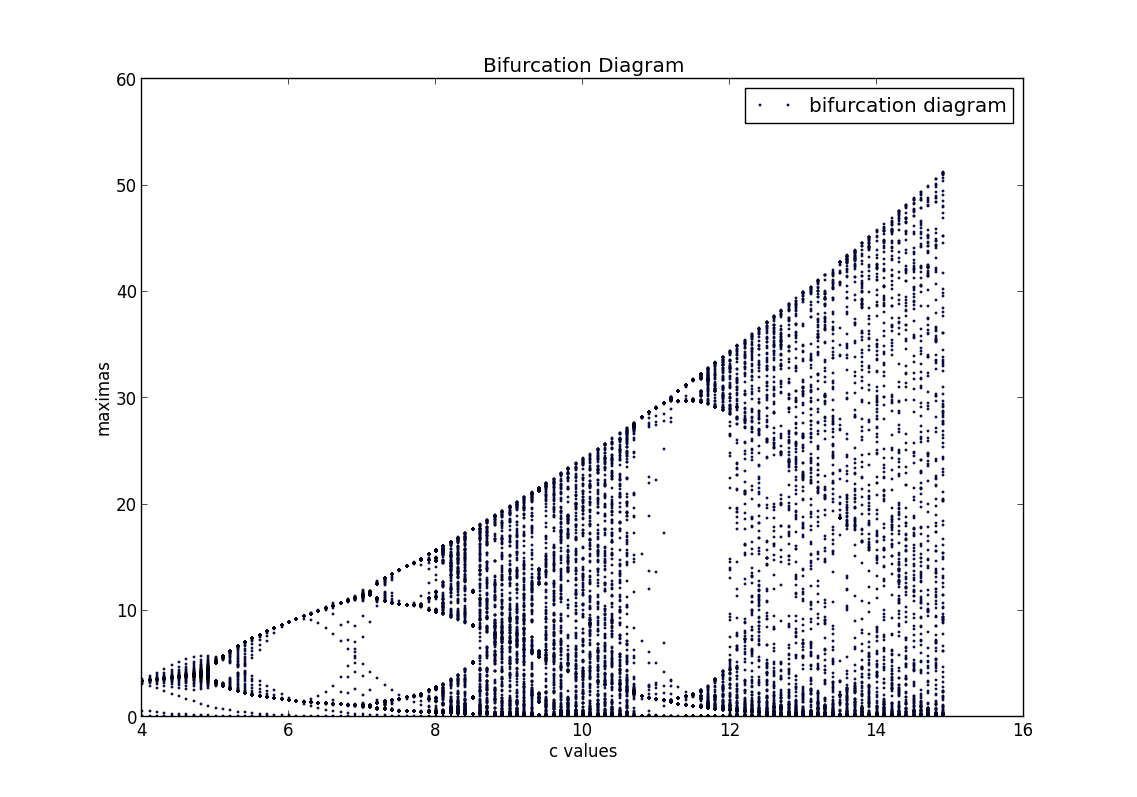
\includegraphics[scale=0.6]{1_d.png}
\caption{Bifurcation Diagram}
This figure shows bifurcation diagram for about 120 c values between 4 and 15. The time interval
\end{figure}
\FloatBarrier

%Section E
\subsection{}

\FloatBarrier
\begin{figure}[h!]
\centering
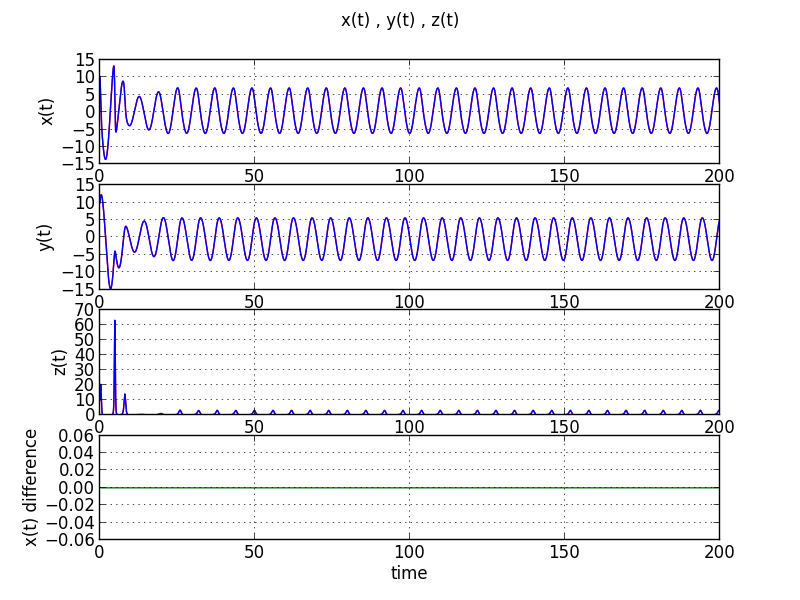
\includegraphics[scale=0.7]{1_e_zero.png}
\caption{Bifurcation Diagram}
This figure shows two Rossler systems plotted simultaneously with exactly the same initial conditions; therefore, the last plot, which is the plot of the difference between x(t) and x1(t) is zero and the other plots are perfectly overlapped.
\end{figure}
\FloatBarrier


\FloatBarrier
\begin{figure}[h]
\centering
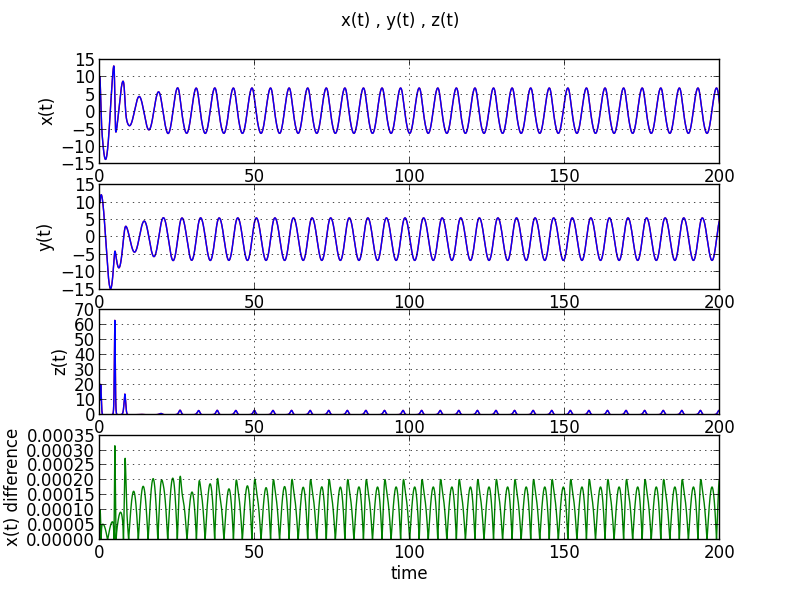
\includegraphics[scale=0.7]{1_e_4.png}
\caption{Bifurcation Diagram}
This figure shows two Rossler systems with the same initial conditions except for x1(0) which is 0.001 off from x(0). C value is 4.
\end{figure}
\FloatBarrier


\FloatBarrier
\begin{figure}[h]
\centering
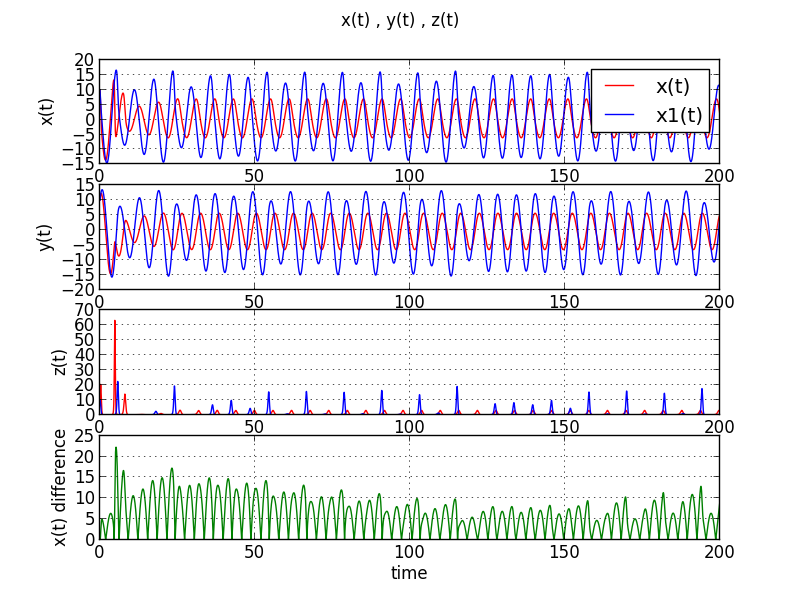
\includegraphics[scale=0.7]{1_e_10.png}
\caption{Bifurcation Diagram}
This figure shows two Rossler systems with the same initial conditions except for x1(0) which is 0.001 off from x(0). C value is 10.
\end{figure}
\FloatBarrier

%Section F
\subsection{}
In this part, I calculated the Lyapunov exponent for the two cases that we looked at in part e(c=4 and c=10) by plotting log|x1-x| for each c where x1 and x are the two slightly different trajectories I plotted in part e. We should only consider the time shortly after the simulation since 

\FloatBarrier
\begin{figure}[h!]
\centering
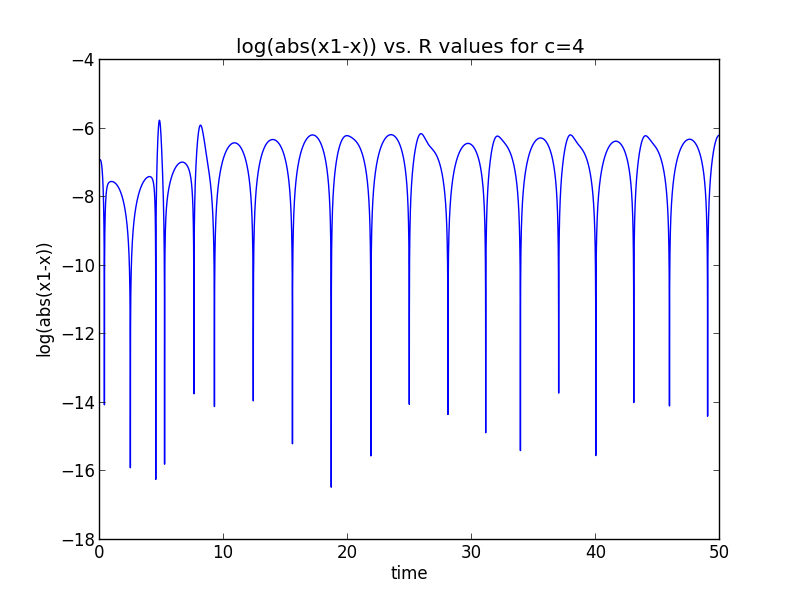
\includegraphics[scale=0.7]{1_f_4.png}
\caption{Lyapunov exponent, c=4}
This figure shows two Rossler systems with the same initial conditions except for x1(0) which is 0.001 off from x(0). C value is 10.
\end{figure}
\FloatBarrier

\FloatBarrier
\begin{figure}[h!]
\centering
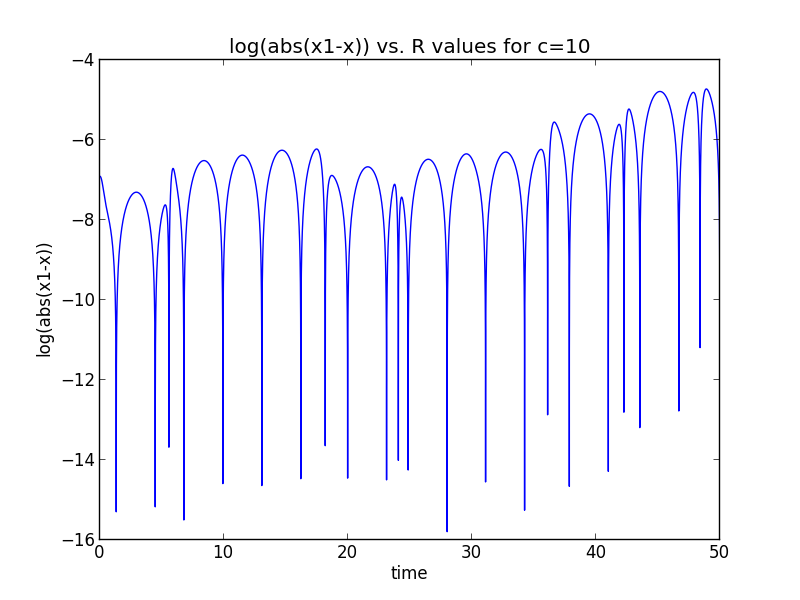
\includegraphics[scale=0.7]{1_f_10.png}
\caption{Lyapunov exponent c=10}
This figure shows two Rossler systems with the same initial conditions except for x1(0) which is 0.001 off from x(0). C value is 10.
\end{figure}
\FloatBarrier



%Question 2
\section{Numerical Methods}
\label{sec:numericalmethods}
In this question, we will use two different methods for plotting the theta and energy of a pendulum called forward Euler method and Euler-Cromer method. Forward Euler method is shown below:

\begin{equation}
v_{i+1}=v_{i}+\Delta \frac{F(t_{i},x_{i},v_{i})}{m}
\end{equation}

\begin{equation}
x_{i+1}=x_{i}+\Delta tv_{i}
\end{equation}


\subsection{}In this part, I used forward Euler method to solve a non-linear pendulum equation which is the following: 

\begin{equation}
\frac{d^2\theta}{dt^2}=-sin\theta 
\end{equation}

Figures 12 shows the plot of \begin{math} \theta \end{math} and energy as a function of time for 60\begin{math} \tau \end{math} respectively, with time step of 0.05\begin{math} \tau \end{math}. As time goes on, the range of theta values becomes larger and larger until it keeps going to the negative or positive part of the plot depending on the initial conditions and never comes back again. As for the energy, it starts from the negative part of the plot and keeps increasing without any bound. I used both \begin{math} \theta \end{math} and derivative of \begin{math} \theta \end{math} to be 1.0 .
Figure 13 shows the same plot as figure ;however, the time step is 0.01\begin{math} \tau \end{math} instead of 0.05 as the previous one. What we see is that theta drops to the negative or positive part of the plot with almost no oscillations, whereas energy gains oscillations as we decreased the time step.
Non of these plots make sense since the energy is not conserved in this case and the system gains energy over time which provokes the physics laws.
%energy and theta vs time plot
\FloatBarrier
\begin{figure}[h!]
\centering
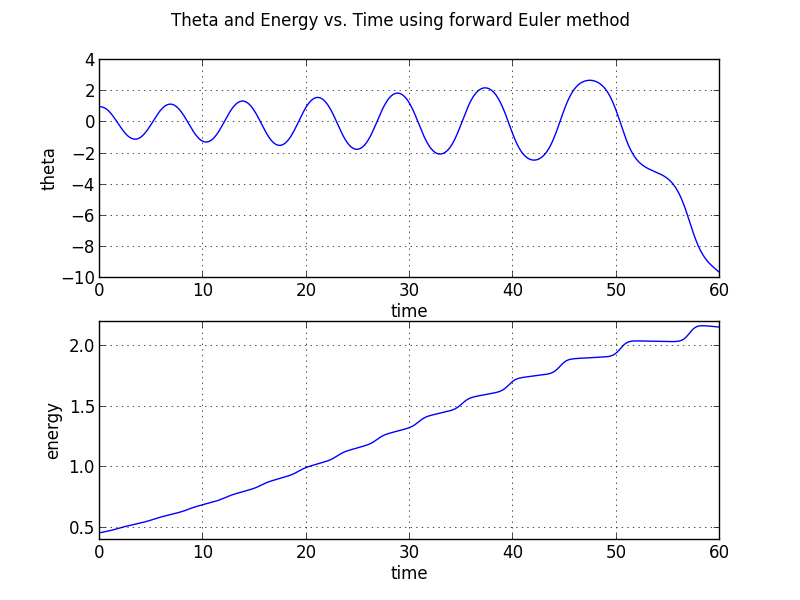
\includegraphics[scale=0.7]{2_a.png}
\caption{Energy and Theta using Forward Euler Method with 0.05 time step}
This figure shows the theta and energy of a pendulum plotted using forward Euler method.
\end{figure}
\FloatBarrier

\FloatBarrier
\begin{figure}[h!]
\centering
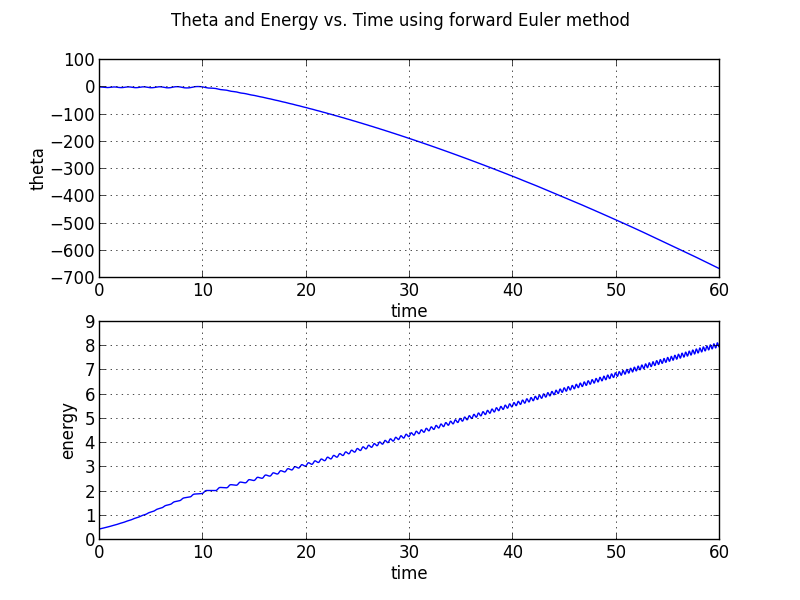
\includegraphics[scale=0.7]{2_a_01.png}
\caption{Energy and Theta using Forward Euler Method with 0.01 time step}
This figure shows the theta and energy of a pendulum plotted using forward Euler method.
\end{figure}
\FloatBarrier


%part b
\subsection{}
In this part I used Euler-Cromer method.  This method is the following:

\begin{equation}
v_{i+1}=v_{i}+\Delta \frac{F(t_{i},x_{i},v_{i})}{m}
\end{equation}

\begin{equation}
x_{i+1}=x_{i}+\Delta tv_{i+1}
\end{equation}

In this method, instead of using \begin{math}v_{i} \end{math}for iteration of \begin{math}x_{i+1} \end{math}, we use \begin{math}v_{i+1} \end{math}.
The difference we see here is that energy is bounded in this method and also theta does not increase or decrease unbounded. Both theta and energy oscillate with constant period and the motion is not periodic.

\FloatBarrier
\begin{figure}[h!]
\centering
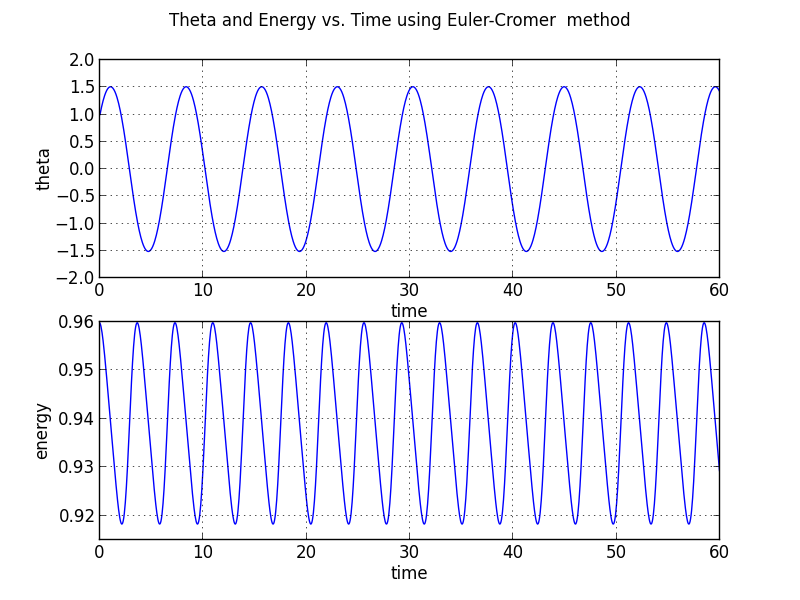
\includegraphics[scale=0.7]{2_b_05.png}
\caption{Energy and Theta using Forward Euler Method with 0.05 time step}
This figure shows the theta and energy of a pendulum plotted using forward Euler method.
\end{figure}
\FloatBarrier


\FloatBarrier
\begin{figure}[h!]
\centering
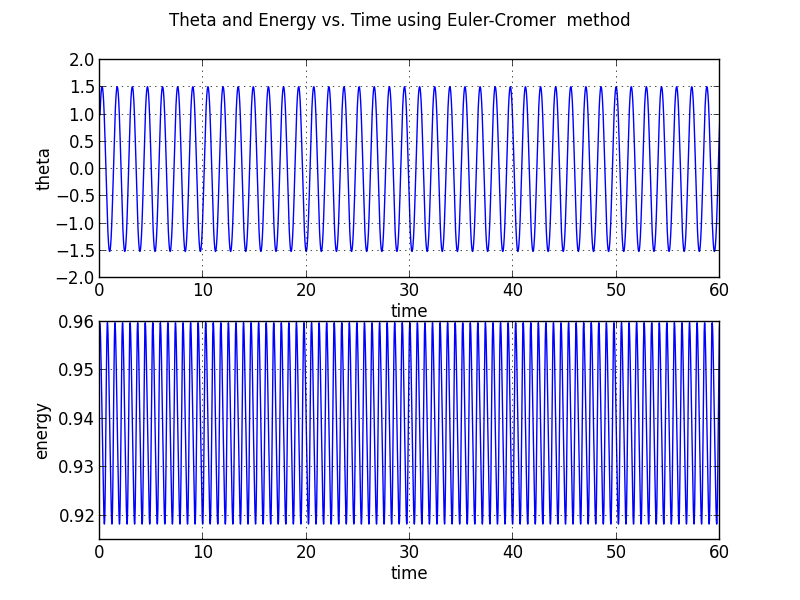
\includegraphics[scale=0.7]{2_b_01.png}
\caption{Energy and Theta using Forward Euler Method with 0.01 time step}
This figure shows the theta and energy of a pendulum plotted using forward Euler method.
\end{figure}
\FloatBarrier

As the instruction handout mentioned, we can see that the numerical method matters. The forward Euler method won't fail in all circumstances, it just happens to be particularly not suitable for problems that have oscillatory motion. Similarly, Euler-Cromer method is not good for all circumstances either, it just happens to be relatively easy to implement.


\subsection{}
Energy varies in this plot. I calculated the maximum and minimum of energy and I took their difference and it happened to be 6.2734221306648408e-07 . This is the highest variation in energy, which is the highest error in numerical method since the energy should be conserved.

\section{The Spring Pendulum}
\label{sec:thespringpendulum}

\subsection{}
According to the figure, we can see the following equations are true:

\begin{equation}
\sin\theta\ = \frac{x}{\acute{l}}
\end{equation}

\begin{equation}
\cos\theta = \frac{l-y}{\acute{l}}
\end{equation}

\begin{equation}
\acute{l}=\sqrt{x^2 + (l-y)^2}
\end{equation}

Forces can be splitter into x and y directions:
Equation 12 is in x-direction while equation 13 is in y-direction.
\begin{equation}
-k(x-l_{0})\sin\theta = m\frac{d^2x}{dt^2} 
\end{equation}

\begin{equation}
-k(l-y)\cos\theta-mg = m\frac{d^2y}{dt^2} 
\end{equation}
And if we divide both sides by m and substitute for \begin{math}\cos\theta and \sin\theta \end{math}, we end up getting the desired equations which are:

\begin{equation}
\frac{d^2y}{dt^2} = -g + \frac{k}{m}(l-y) - \frac{k}{m} l_{0}\frac{(l-y)}{\sqrt{x^2 + (l-y)^2}}
\end{equation}

\begin{equation}
\frac{d^2x}{dt^2} =- \frac{k}{m}x + \frac{k}{m}\frac{l_{0}x}{\sqrt{x^2 + (l-y)^2}}
\end{equation}

\subsection{}
We use equation 14 to substitute values in. We have the following equations:

\FloatBarrier
\begin{figure}[h!]
\centering
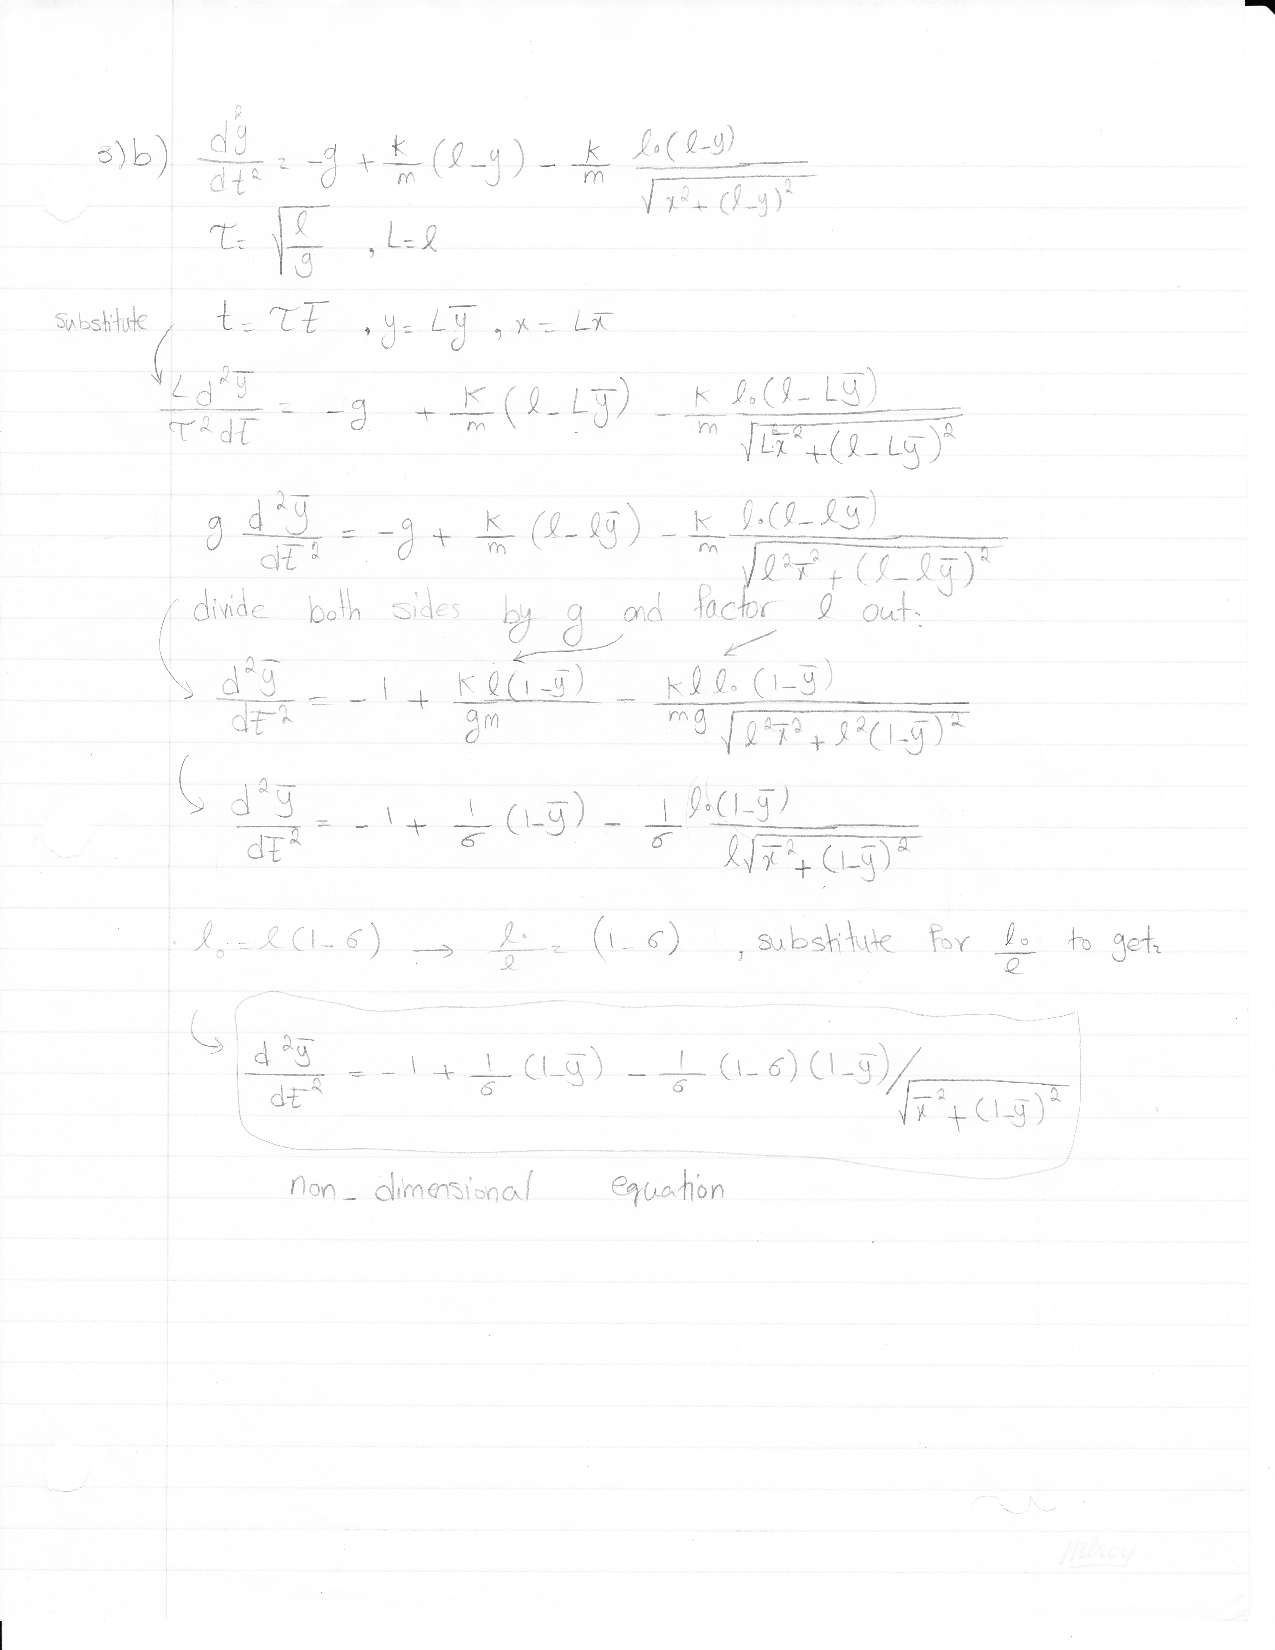
\includegraphics[scale=0.6]{3_b_1.pdf}
\caption{Spring Pendulum Solved Numerically using odeint}

\end{figure}
\FloatBarrier



\FloatBarrier
\begin{figure}[h!]
\centering
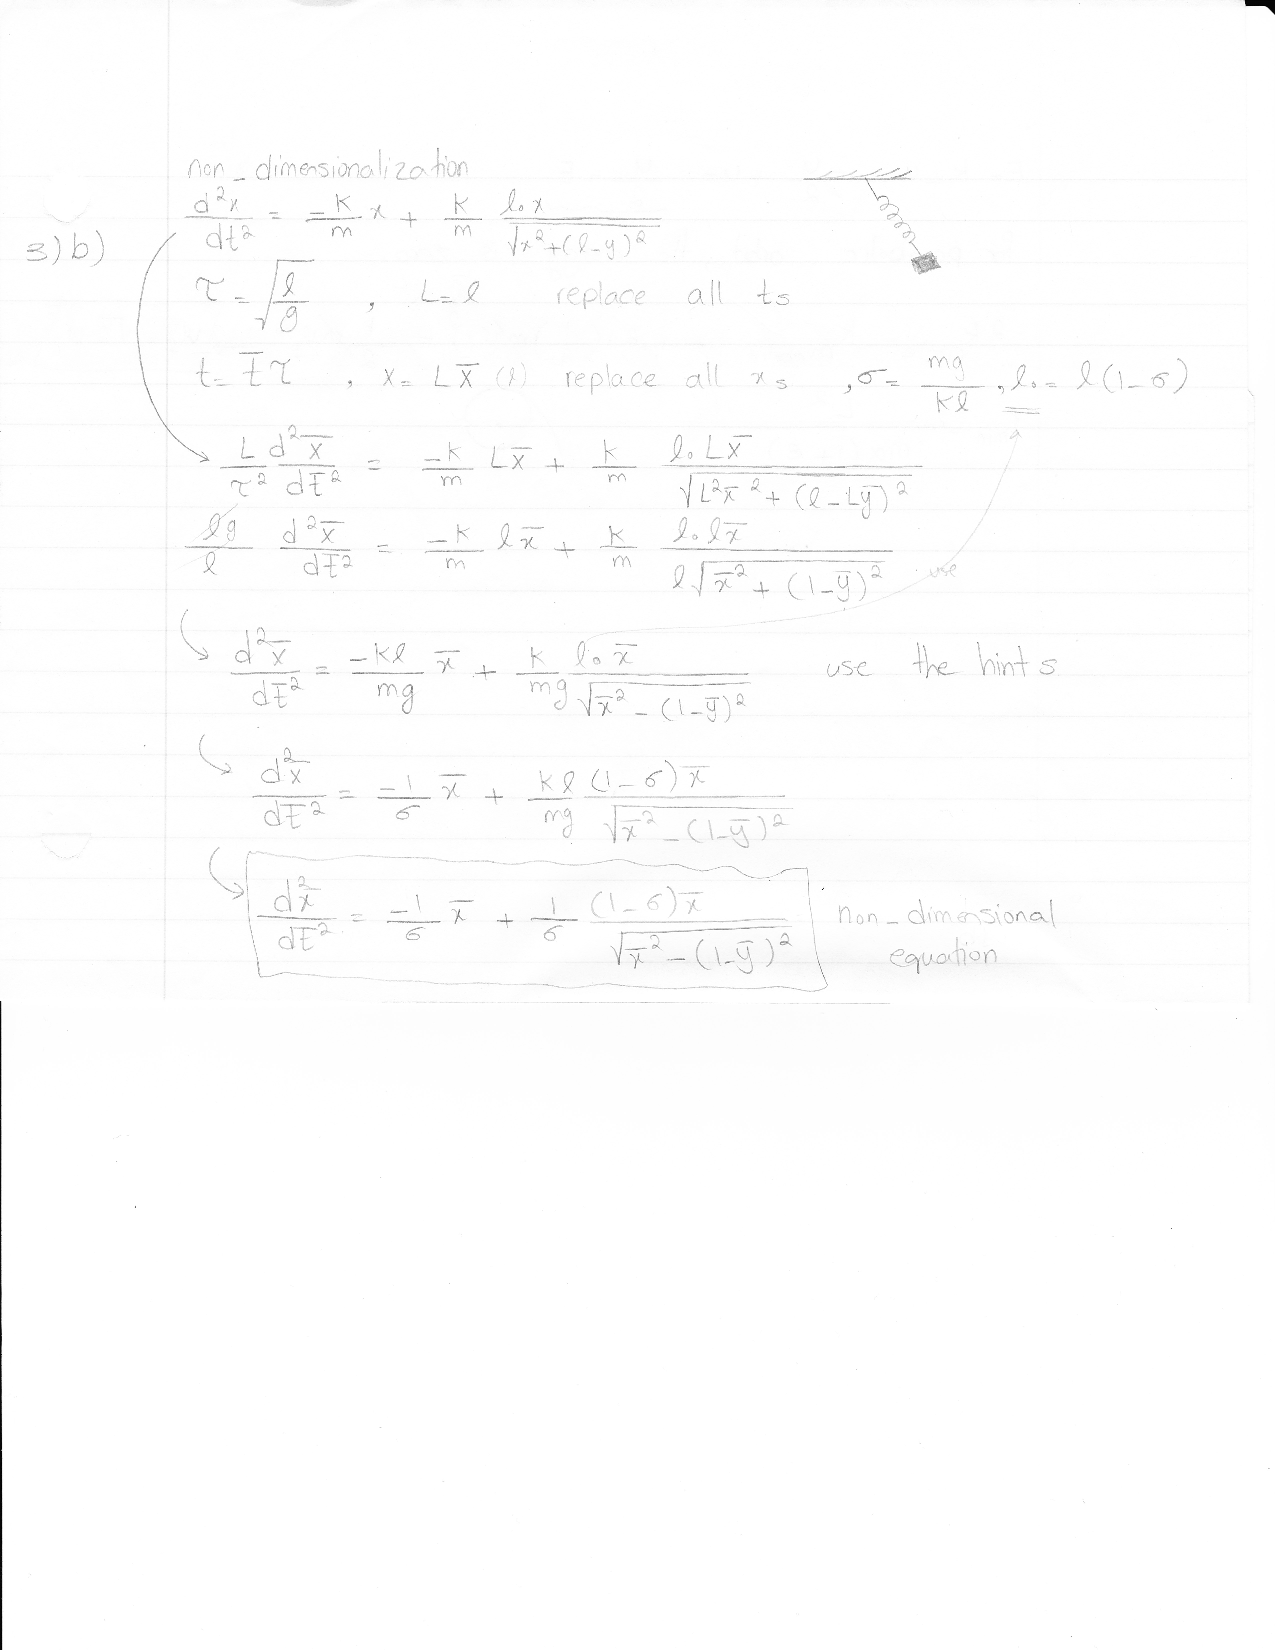
\includegraphics[scale=0.7]{3_b_2.pdf}
\caption{Non-dimensional equations}

\end{figure}
\FloatBarrier


\FloatBarrier
\begin{figure}[h!]
\centering
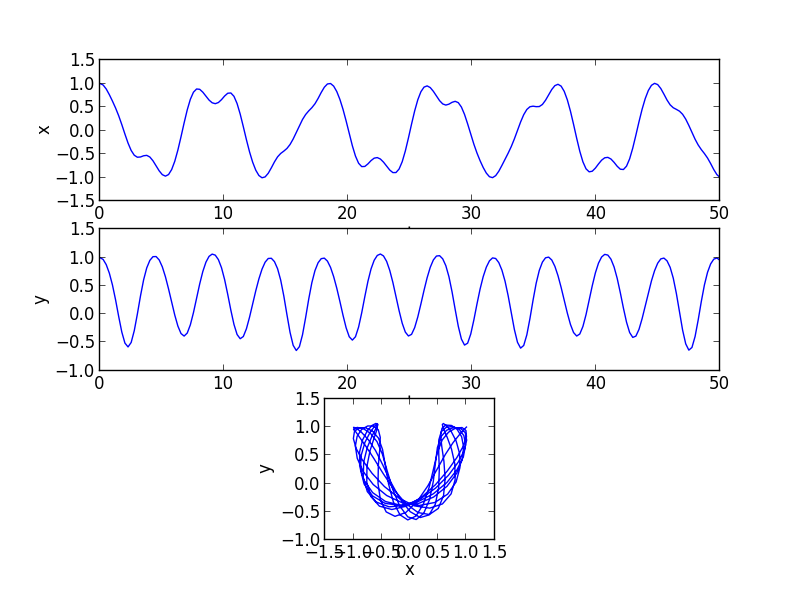
\includegraphics[scale=0.7]{3_c.png}
\caption{Non-dimensional equations}

\end{figure}
\FloatBarrier

\subsection{}
In this part, we only need to type the non-dimensional equations we got in part b. By plugging in the equations and also the initial values in, \begin{math} x_{0}=y_{0}=1 , \frac{dx}{dt}=\frac{dy}{dt}=0\end{math}. It runs for 50 seconds with 200 values in between so there is a time step of 0.25 . 

\subsection{}
\begin{math}\sigma\end{math} is a non-dimensional parameter in our equations. 
\begin{equation}
\sigma = \frac{mg}{kl}
\end{equation}

Setting \begin{math}\sigma\end{math}  to be 0.0001, results in the following image:
Other initial conditions have the values of \begin{math}x_{0}=0.8, y_{0}=0.4  \end{math} and \begin{math} v_{x_{0}}=v{y_{0}}=0.\end{math}

\FloatBarrier
\begin{figure}[h!]
\centering
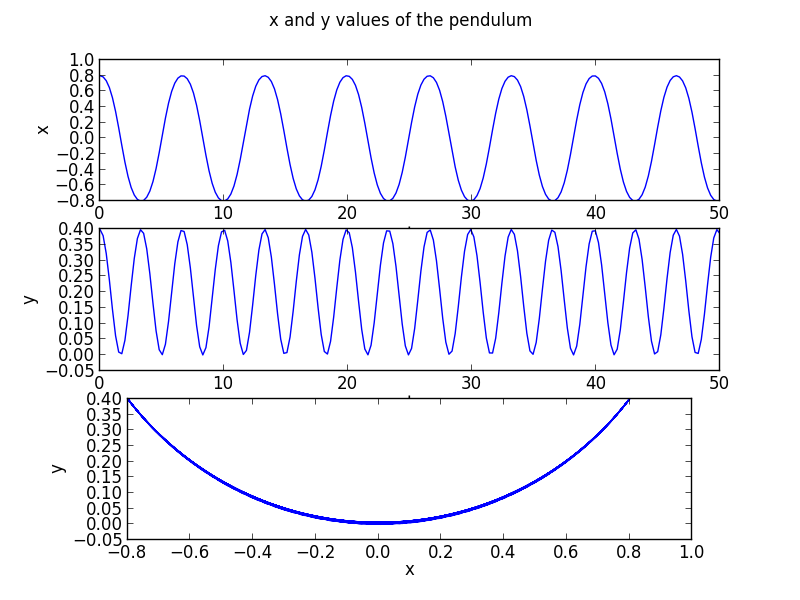
\includegraphics[scale=0.7]{3_d.png}
\caption{sigma set to be 0.0001}
\end{figure}


What happens for very small sigma is that the y versus x diagram is part of a parabola and repeats itself, meaning the system is not chaotic for very small sigma. The path would just go on itself again and again, whereas in larger sigma values, the pattern does not repeat itself meaning the system is chaotic for larger sigma values.

\FloatBarrier

\end{document}